\documentclass[tikz,border=5mm]{standalone}
\usepackage{pgfplots}
\usepackage{amsmath}
\pgfplotsset{compat=1.18}

\begin{document}
	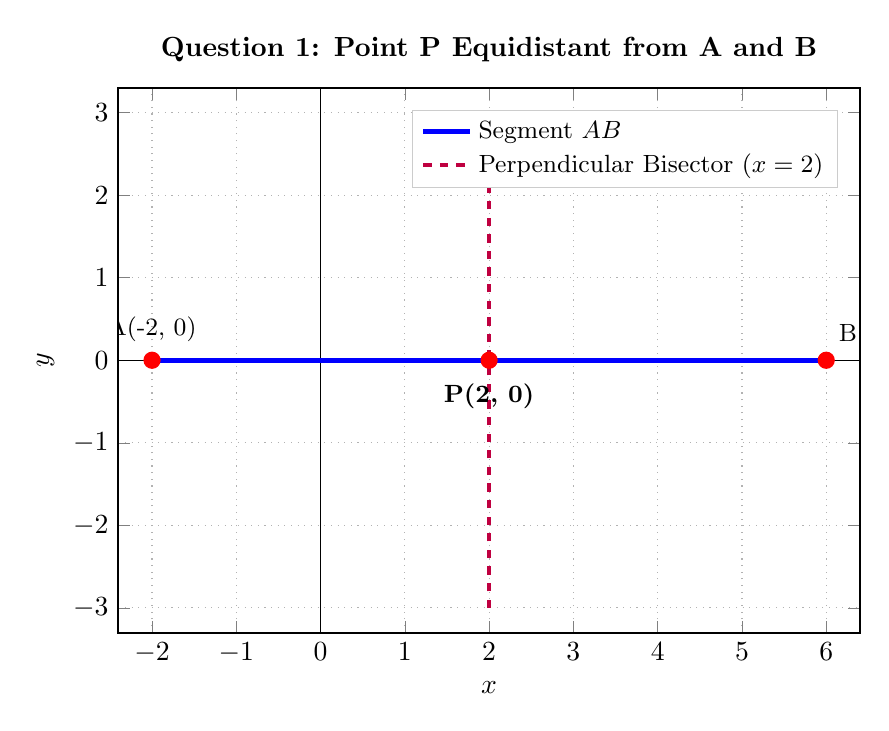
\begin{tikzpicture}
		\begin{axis}[
			width=11cm, height=8.5cm,
			title={\textbf{Question 1: Point P Equidistant from A and B}},
			xlabel={$x$}, ylabel={$y$},
			xmin=-2.4, xmax=6.4,
			ymin=-3.3, ymax=3.3,
			xtick={-2,-1,0,1,2,3,4,5,6},
			ytick={-3,-2,-1,0,1,2,3},
			grid=both,
			grid style={dotted, gray!60},
			axis line style={black, thick},
			legend cell align={left},
			legend style={at={(0.97,0.96)}, anchor=north east, font=\small, draw=gray!40}
			]
			% Axes lines (x=0, y=0)
			\draw[black, thin] (axis cs:0,-3.3) -- (axis cs:0,3.3);
			\draw[black, thin] (axis cs:-2.4,0) -- (axis cs:6.4,0);
			
			% Segment AB
			\addplot[blue, line width=1.8pt] coordinates {(-2,0) (6,0)};
			\addlegendentry{Segment $AB$}
			
			% Perpendicular Bisector (x = 2)
			\addplot[purple, dashed, line width=1.4pt] coordinates {(2,-3) (2,3)};
			\addlegendentry{Perpendicular Bisector ($x = 2$)}
			
			% Points A, P, B
			\node[circle, fill=red, inner sep=2.2pt] at (axis cs:-2,0) {};
			\node[above=3pt, font=\small] at (axis cs:-2,0) {A(-2, 0)};
			
			\node[circle, fill=red, inner sep=2.2pt] at (axis cs:6,0) {};
			\node[above right=1pt, font=\small] at (axis cs:6,0) {B(6, 0)};
			
			\node[circle, fill=red, inner sep=2.2pt] at (axis cs:2,0) {};
			\node[below=5pt, font=\small\bfseries] at (axis cs:2,0) {P(2, 0)};
		\end{axis}
	\end{tikzpicture}
\end{document}